\chapter{Marco teórico}\label{chap:Marcoteorico}


\section{Brazos robóticos industriales}

Antes de entrar en el tema principal de este documento, es importante conocer el antecedente o lo que se trata de mejorar, en nuestro caso, es imposible hablar de robots colaborativos sin primero abordar los brazos robóticos industriales.

Un brazo robótico es un manipulador, usualmente programable con funciones similares a las de un brazo humano. Los eslabones de este manipulador estan conectados por articulaciones que permiten el movimiento rotacional o translacional \cite{ReviewRoboticArm} \cite{Schilling2001}.

Diversos autores concuerdan que el primer brazo robótico industrial se instaló en una cadena de montaje de la empresa automotriz General Motors, fue presentado en 1961 y llevó por nombre Unimate, para despúes conocerse como a PUMA. Otros notorios desarrollos notorios se dieron en 1963 con el diseño del brazo robótico Rancho, en 1969 cuando Victor Scheinman desarrolló el brazo Stanford y en 1974 se desarrolló el brazo robótico Silver del MIT \cite{Moran2007}.


\subsection{Clasificación de los brazos robóticos}

De acuedo con \cite{Gupta2016}, los brazos robóticos pueden clasificarse por cuatro elementos fundamentales de operación.

\begin{itemize}
\itemsep0em
\item Por su sistema coordenado
\item Por su fuente de energía
\item Por su método de control
\item Por su método de programación
\end{itemize}

\subsubsection{Clasificación por su sistema coordenado}


\paragraph{Cartesianos.} Un manipulador cartesiano tiene la configuración más sencilla. La imagen \ref{fig:robotcartesiano} muestra un ejemplo, donde podemos observar tres articulaciones \textit{prismáticas} mutuamente ortogonáles \cite{Craig2013}. Algunos autores llaman a esta configuración de robots x-y-z, por los ejes de movimiento.

Debido a su simple forma, esta configuración posee la ventaja de una gran robustez, lo que facilita poder construir máquinas de gran tamaño y con una carga útil elevada.

\begin{figure}
    \centering
    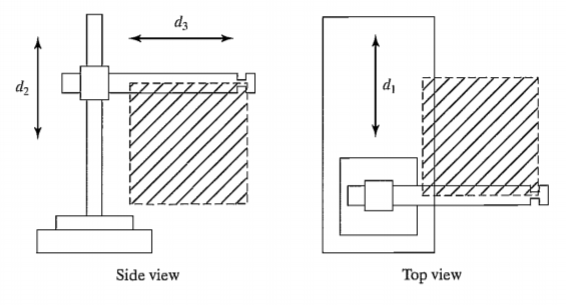
\includegraphics[scale=0.8]{./img/chapter2/cartesiano.png}
    \caption{Robot cartesinao}
    \label{fig:robotcartesiano}
\end{figure}

Ejemplos de esta configuración los podemos observar en máquinas CNC como cortadoras láser, impresoras 3D o en máquinas \textit{pick and place}. 


\paragraph{Cilíndricos.} Los manipuladores cilíndricos se forman con una articulación de tipo \textit{revoluta} en conjunto con dos articulaciones prísmáticas, una de ellas para moverse en el eje vertical y otra con un movimiento ortogonal a la articulación del tipo revoluta.

Un ejemplo de esta configuración se puede apreciar en la figura \ref{fig:robotcilindrico}.

\begin{figure}
    \centering
    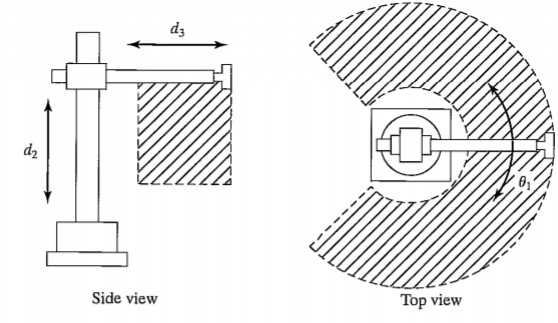
\includegraphics[scale=0.8]{./img/chapter2/cilindrico.png}
    \caption{Robot cilíndrico}
    \label{fig:robotcilindrico}
\end{figure}

Las aplicaciones de este tipo de robots son en atender maquinaria, operaciones de ensamblado y en soldadura de punto.

Sus ventajas son que tiene un área de trabajo extendida, puede alcanzar puntos alrededor de su ubicación y es lo suficinetemente robusta para mover cargas pesadas a lo largo de su área de trabajo. 

Las desventajas de esta configuración es que no puede moverse a través de obstáculos en su área de trabajo y no puede alcanzar puntos ariba de ella misma. 

\paragraph{Esféricos.} 

\begin{figure}
    \centering
    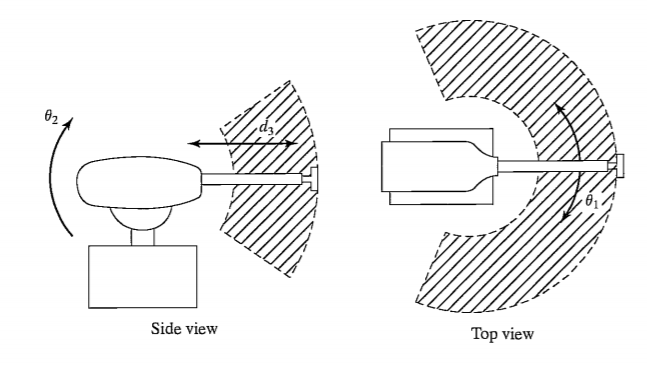
\includegraphics[scale=0.8]{./img/chapter2/esferico.png}
    \caption{Robot esférico}
    \label{fig:robotesferico}
\end{figure}

\paragraph{Articulado.}

\begin{figure}
    \centering
    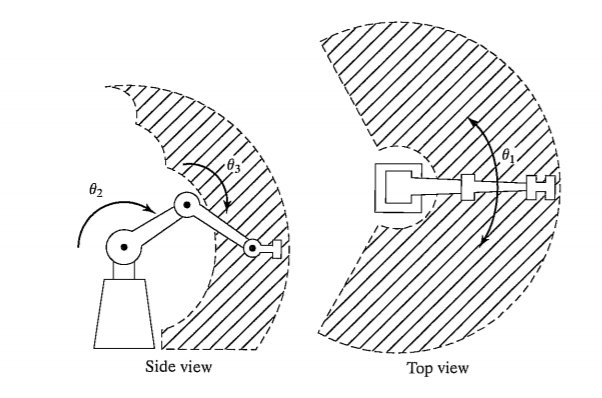
\includegraphics[scale=0.8]{./img/chapter2/articulado.png}
    \caption{Robot articulado}
    \label{fig:robotarticulado}
\end{figure}

\paragraph{SCARA.}

\begin{figure}
    \centering
    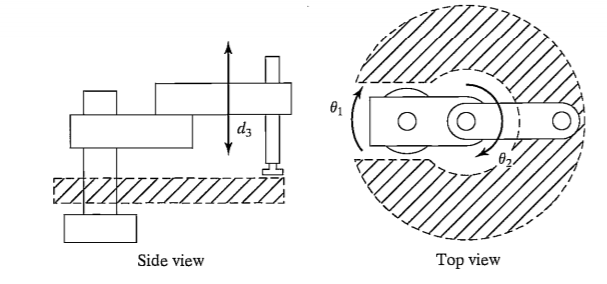
\includegraphics[scale=0.8]{./img/chapter2/scara.png}
    \caption{Robot SCARA}
    \label{fig:robotscara}
\end{figure}

\subsubsection{Clasificación por su fuente de energía}

La energía necesaria para mover las articulaciones y eslabones de un brazo robótico pueden venir de diferentes fuentes. En la actualidad, existen tres principales fuentes de energía para un brazo robótico. A continuación se mencionan.

\begin{itemize}
\itemsep0em
\item Energía hidráulica
\item Energía neumática
\item Energía eléctrica
\end{itemize}

\paragraph{Energía hidráulica.} Es la fuente de energía más popular, debido principalmente a que sus motores y cilindros son pequeños y producen fuerza y torque elevados, de igual manera, pude poseer un sistema de control preciso. 

Estos sistemas funcionan por un fluido que es  bombeado a través de los morores, cilindros u otros actuadores hidráulicos, convirtiendo las fuerzas de la alta presión en movimiento rotacional o lineal.

Las ventajas de estos robots se centran en su gran poder de salida sin la necesidad de usar engranes reductores, así como su uso en ambientes donde utilizar energía eléctrica podría causar incendios o explosiones. 

\paragraph{Energía neumática.}  Según \cite{Craig2013}, los sistemas neumáticos se encuentran en 30\% de los robots de hoy en día. Estos sistemas usan aire comprimido para suministrar la energía. La popularidad de estos brazos robóticos se da debido a que la mayoría de las industrias ya cuentan con lineas de aire comprimido antes de pensar en un brazo robótico.

Las ventajas de un brazo robótico energizado con energía neumática es su costo más barato que las demás alternativas pues la matería prima es gratis, no contaminan el área de trabajo con aceites y tienen un tiempo de respuesta más rápido que los sistemas hidráulicos.

Su desventaja principal es que el control no es tan preciso y, por lo regular, se diseñan con menos grados de libertad. 

\paragraph{Energía eléctica.} La energía eléctrica usa servomotores, motores a pasos y motores de corriente continua, los cuales convierten la energía eléctrica en energía mecánica.

Comparado con los sistemas hidráulicos, los sistemas eléctricos proveen menos fuerza y velocidad, pero son mucho mejores en precisión y repetitibilidad.

Existen tres tipos principales de mootores eléctricos comúnmente usados en robots:

\begin{itemize}
\itemsep0em
\item Motores a pasos. Son motores baratos, usados principalmente en máquinas pick an place donde la carga útil no es tan grande y se requiere un control lo suficientemente preciso.

\item Servomotores de corriente directa. Ofrecen buena potencia de salida con un alto grado de de control de la posición y velocidad. 

\item Servmomotres de corriente alterna sin escobillas. El estandar a utilizar hoy en día, ofrecen una potencia de salida mayor a los servomotores de corriente directa y son bastante silenciosos. Al no tener escobillas requieren practicamente cero mantenimiento.
\end{itemize}



\subsubsection{Clasificación por su método de control}
\subsubsection{Clasificación por su método de programación}



\subsection{Anatomía de un brazo robótico articulado}

Está claro que la inspiración del brazo robótico viene de la anatomía humana, así que es lógico que las partes del robot se nombren como las partes similares de la anatomía humana.

A continuación, se mencionan con mayor profundidad las partes de un brazo robótico, de igual manera, en la figura \ref{fig:anatomiadeunbrazo}, se hace una demostración visual de la analogía utilizada.

\begin{figure}
    \centering
    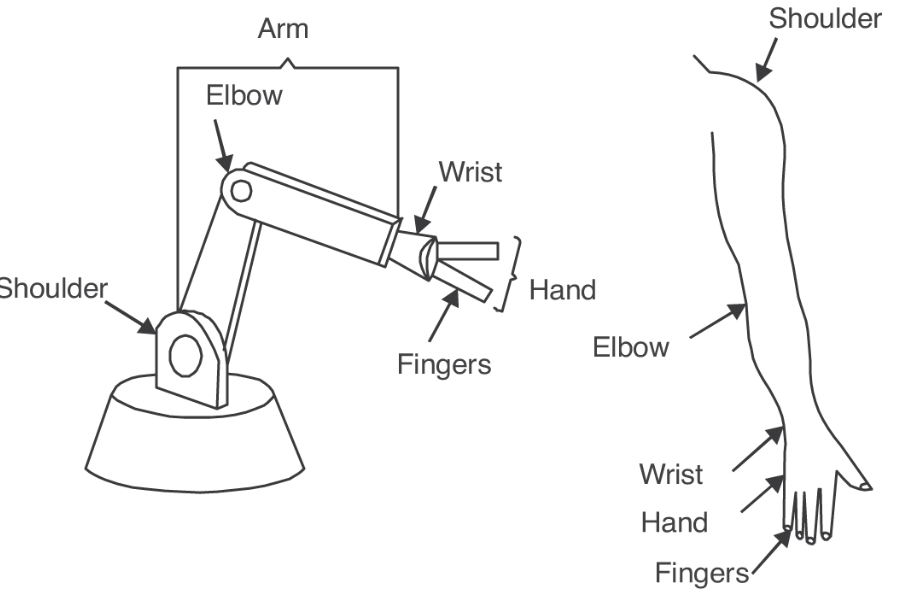
\includegraphics[scale=0.8]{./img/chapter2/anatomiabrazo.png}
    \caption{Anatomía de un brazo robótico \cite{Gupta2016}.}
    \label{fig:anatomiadeunbrazo}
\end{figure}

\paragraph{Hombro.} 



\subsubsection{Codo}
\subsubsection{Muñeca}
\subsubsection{Mano}


\subsection{Terminología de un brazo robótico}




\subsection{Efector final}


\section{Robótica colaborativa}

La robótica colaborativa surge como una rama de la robótica dispuesta a hacer más fácil el trabajo en lineas de producción, así como aliviar problemas en la espalda relacionados con tareas de ensamblado final en posiciones no ergonómicas \cite{cobot2018}\cite{cobotreview}.

Los robots colaborativos han sido desarrollados para trabajar de manera segura al lado de humanos, tomando en consideración la seguridad del operador, la del mismo robot y la correcta realización de la tarea a realizar.  Por esto, están equipados con medidas de seguridad para reconocer el ambiente en el que trabajan, tales como sistemas de evasión de obstáculos y detección de colisiones, implementadas a través de sensores o de mecanismos de compilación pasiva.

\paragraph{Escenarios de colaboración.} Es claro que no todas las aplicaciones donde se implemente un robot colaborativo requieren las mismas consideraciones, es por esto que existe una clasificación de acuerdo al grado de interacción con el operador y la dependencia entre éste y el robot colaborativo. Esos escenarios se mencionan a continuación y se ilustran en la figura \ref{fig:escenarioscolaborativos} \cite{Zaatari2019}.


\begin{itemize}
\itemsep0em
\item \textbf{Independiente.} Un operador y un robot colaborativo trabajan en distintas piezas de trabajo, cada uno con un proceso de manufactura individual. El elemento colaborativo es debido a la co-presencia en la misma área de trabajo.
\item \textbf{Simultanea.} Un operador y un robot colaborativo operan en procesos separados en la misma pieza de trabajo al mismo tiempo. No existe una dependencia de tarea entre ellos, sin embargo, el cobot debe estar conciente y respetar el espacio del operador.
\item \textbf{Secuencial.} Un operador y un cobot relizan un proceso de manufactura secuencial en la misma pieza de trabajo. Existe dependencia de tiempo entre ambos a lo largo del proceso.
\item \textbf{Soporte.} Un operador y un robot trabajan en el mismo proceso de manera interaciva. Existe una dependencia entre las acciones del robot y el operador, es decir, sin uno de ellos, la tarea no podría realizarse.
\end{itemize}

\begin{figure}
    \centering
    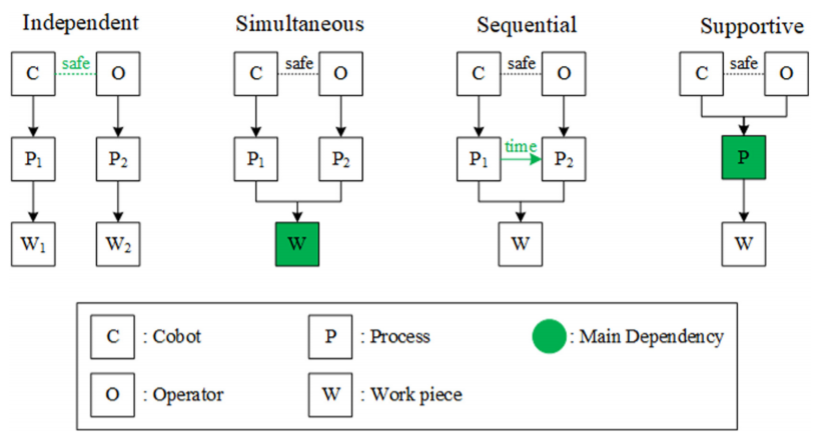
\includegraphics[scale=0.8]{./img/chapter2/escenarioscolaborativos.png}
    \caption{Escenarios colaborativos}
    \label{fig:escenarioscolaborativos}
\end{figure}

Con esto en mente, es fácil deducir que la mayoría de las investigaciones en el área de robótica colaborativa están encaminadas a estudiar o mejorar la detección de colisiones para salvaguardar la integridad de las personas que deberán trabajar junto a los cobots.

Incluso antes de que se acuñara el término cobots, ya había investigaciones encaminadas a la evasión de obstáculos \cite{Khatib1986}, dónde se plantea la solución a través de algoritmos de planeación de ruta.


En la mayoría de los robots colaborativos que existen en el mercado hoy en día se utilizan sensores de fuerza-torque en cada una de las articulaciones, sin embargo, los sensores montados en el robot colaborativo no son la única forma de proveer la seguridad necesaria, en \cite{Teke2018}, se aborda el uso de sensores de visión computacional a través del dispositivo Kinect V2 de Microsoft para modificar la trayectoria y así evadir obstáculos.

En \cite{Lu2005}, se concluye que es posible detectar colisiones utilizando sensores de fuerza-torque únicamente en la base y muñeca de un brazo robótico. Los sensores de fuerza-torque son sumamente caros, por esta razón existen investigaciones como \cite{Phan2018} donde se trabaja en desarrollar nuevos sensores de fuerza-torque con gran velocidad de respuesta y bajo costo.

De igual forma, se han desarrollado estudios sobre como es posible desarrollar robots colaborativos sin la necesidad de sensores de fuerza-torque.

En \cite{Matsumotoa}, se propone un método de detección de colisión basado en la ley de control no-lineal adaptativo, donde se utiliza la diferencia entre el torque obtenido realmente en contra del calculado basado en el modelo dinámico.

Por otra parte, en \cite{Chen2018} también se propone el desarollo de un algoritmo de detección de colisión basado en el modelo dinámico del robot, en este se utiliza la corriente suministrada al motor y la información que proporcionen los sensores de posición para medir discrepancias y detectar colisiones, lo que reduce el costo dedicado a sensores que requiere un robot colaborativo. En esta investigación se tratará de replicar esta metodología para lograr un algoritmo de detección de colisión.

Uno de los ejemplos más populares de robots colaborativos es la línea de robots UR creada por Universal Robots, quién ha vendido más de 39,000 unidades de estos cobots. Una imagen del mismo puede ser apreciada en la figura \ref{fig:ur5}.


\subsection{Seguridad}

\begin{figure}
    \centering
    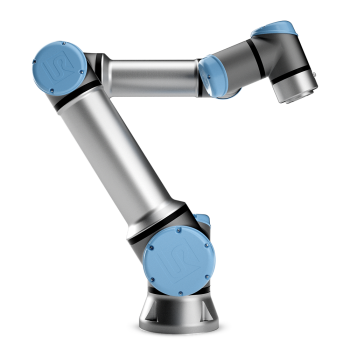
\includegraphics[scale=0.5]{./img/chapter2/ur5.png}
    \caption{Robot colaborativo UR5 de Universal Robots}
    \label{fig:ur5}
\end{figure}

\section{Diseño de un brazo robótico}
\subsection{Actuadores}\label{sec:actuadores}

\cite{Pham2018} - Review de actuadores.

\subsubsection{Engranes planetarios}
\subsubsection{Harmonic Drive}
\subsubsection{Engrane cicloidal}

En \cite{Sensinger2012} se concluye que un engrane cicloidal se debería usar en aplicaciones antropomórficas donde el tamaño y el toeque tengan preferencia ....

\section{Manufactura aditiva}

